\documentclass[runningheads,a4paper,11pt]{report}

\usepackage{algorithmic}
\usepackage{algorithm} 
\usepackage{array}
\usepackage{amsmath}
\usepackage{amsfonts}
\usepackage{amssymb}
\usepackage{amsthm}
\usepackage{caption}
\usepackage{comment} 
\usepackage{epsfig} 
\usepackage{fancyhdr}
\usepackage[T1]{fontenc}
\usepackage{geometry} 
\usepackage{graphicx}
\usepackage[colorlinks]{hyperref} 
\usepackage[latin1]{inputenc}
\usepackage{multicol}
\usepackage{multirow} 
\usepackage{rotating}
\usepackage{setspace}
\usepackage{subfigure}
\usepackage{url}
\usepackage{verbatim}
\usepackage{xcolor}
\usepackage{pgfgantt}
\usepackage{tikz}
\usetikzlibrary{arrows.meta,positioning,shapes.multipart,fit}


\geometry{a4paper,top=3cm,left=2cm,right=2cm,bottom=3cm}

\pagestyle{fancy}
\fancyhf{}
\fancyhead[LE,RO]{Medical-Certificates DDE}
\fancyhead[RE,LO]{InnoMind}
\fancyfoot[RE,LO]{ITSG 2025-2026}
\fancyfoot[LE,RO]{\thepage}

\renewcommand{\headrulewidth}{2pt}
\renewcommand{\footrulewidth}{1pt}
\renewcommand{\headrule}{\hbox to\headwidth{%
  \color{lime}\leaders\hrule height \headrulewidth\hfill}}
\renewcommand{\footrule}{\hbox to\headwidth{%
  \color{lime}\leaders\hrule height \footrulewidth\hfill}}

\hypersetup{
pdftitle={artTitle},
pdfauthor={name},
pdfkeywords={pdf, latex, tex, ps2pdf, dvipdfm, pdflatex},
bookmarksnumbered,
pdfstartview={FitH},
urlcolor=cyan,
colorlinks=true,
linkcolor=red,
citecolor=green,
}


\setcounter{secnumdepth}{3}
\setcounter{tocdepth}{3}
\linespread{1}
\makeindex


\begin{document}

\begin{titlepage}
\sloppy

\begin{center}
BABE\c S BOLYAI UNIVERSITY, CLUJ NAPOCA, ROM\^ ANIA

FACULTY OF MATHEMATICS AND COMPUTER SCIENCE

\vspace{6cm}

\Huge \textbf{}

\vspace{1cm}

\normalsize INTELLIGENT DOCUMENT PROCESSING FOR ROMANIAN MEDICAL CERTIFICATES

\end{center}


\vspace{5cm}

\begin{flushright}
\Large{\textbf{Team members}}\\
Nichifor Dragos, IS, 258-2, dragos.nichifor@stud.ubbcluj.ro

Malancioiu Daniel-George, IS, 258-2, daniel.malancioiu@stud.ubbcluj.ro

Lupu Eduard-Adrian, IS, 258-2, eduard.lupu@stud.ubbcluj.ro
\end{flushright}

\vspace{4cm}

\begin{center}
2025-2026
\end{center}

\end{titlepage}

\pagenumbering{gobble}

\begin{abstract}
	Text of abstract. Short info about: 
	\begin{itemize}
		\item project relevance/importance, 
		\item inteligent methods used for solving, 
		\item data involved in the numerical experiments; 
		\item conclude by the the results obtained.
		\item Please add a graphical abstract of your work. 
	\end{itemize}

	

\noindent
\textbf{\textcolor{green}{Remind that a good report should:}}
\begin{itemize}	
	\item be fun to read with many figures and visualizations;
	\item be easy to follow even for AI/ML novice;
	\item clearly convey the potential of AI/ML to the application domain;
	\item around 10 minutes to read (although this is not a hard constraint).
\end{itemize}

\end{abstract}


\tableofcontents

\newpage

\listoftables
\listoffigures
\listofalgorithms

\newpage

\setstretch{1.5}



\newpage

\pagenumbering{arabic}


% ---------------------------------------------------------------------------------------------------------------


\chapter{Team composition and roles}
\label{chapter:team}

\section{Table of main skills and contributions}

\begin{table}[h!]
\centering
\begin{tabular}{|l|p{5cm}|p{6cm}|}
\hline
\textbf{Name} & \textbf{Main Skills} & \textbf{Roles and Contributions} \\ \hline
Nichifor Dragos &
Python development, OpenCV, Streamlit, OCR pipeline design, testing, documentation &
\\ \hline
Malancioiu Daniel-George &
Python development, OpenCV, Streamlit, OCR pipeline design, testing, documentation &
\\ \hline
Lupu Eduard-Adrian &
Python development, OpenCV, Streamlit, OCR pipeline design, testing, documentation &
\\ \hline
\multicolumn{3}{|p{14cm}|}{
\textbf{Note:} All team members shared identical technical responsibilities and actively participated in every project stage.  
Development followed a \textbf{pair programming} and \textbf{peer review} workflow to ensure code consistency and shared understanding.  
Documentation was written collaboratively, with all members contributing to structure, content, and refinement.  
This cooperative approach ensured a balanced workload, and higher software reliability.
} \\ \hline
\end{tabular}
\caption{Team members, shared skills, and collaborative responsibilities.}
\end{table}

\newpage 
\section{Performed tasks (Gantt diagram)}
\addcontentsline{toc}{section}{Performed tasks (Gantt diagram)}

\begin{figure}[htbp]
\centering
\resizebox{\textwidth}{!}{%
\begin{ganttchart}[
  hgrid, vgrid,
  x unit=0.38cm,
  y unit chart=0.50cm,
  bar height=0.45,
  group right shift=0,
  group/.append style={fill=gray!60},
  bar/.append style={fill=gray!30},
  milestone/.append style={fill=black},
  bar label font=\tiny,
  title label font=\scriptsize
]{1}{14}
  \gantttitle{Project Timeline (Weeks)}{14} \\
  \gantttitlelist{1,...,14}{1} \\

  \ganttgroup{\tiny{Planning \& Setup}}{1}{2} \\
  \ganttgroup{\tiny{Implementation}}{2}{4} \\
  \ganttgroup{\tiny{Validation \& Reporting}}{3}{4} \\

  \ganttbar{Lab1}{1}{2} \\ 
  \ganttbar{Lab2}{2}{4} \\
  \ganttbar{Lab3}{3}{4} \\ 
  \ganttbar{Lab4}{4}{4} \\ 
  \ganttbar{Lab5}{4}{4} \\ 
  \ganttbar{Lab6}{4}{4} \\
  \ganttbar{Lab7}{4}{4} \\
\end{ganttchart}
}
\caption{ Compact schedule by lab milestones. }
\end{figure}


% ---------------------------------------------------------------------------------------------------------------


\chapter{Introduction}
\label{chapter:introduction}

\section{What? Why? How?}
\label{section:what}

This report presents an intelligent web-based system designed to automatically extract structured information from Romanian \textbf{medical leave certificates} (\textit{Certificat de Concediu Medical}) issued by CNAS.

The main idea behind the project is to build a practical and lightweight solution that transforms scanned or photographed documents into digital records containing key fields such as \texttt{Series}, \texttt{Number}, \texttt{CNP},  \texttt{Start Date}, \texttt{End Date}, and \texttt{Diagnostic Code}.  
The application provides an end-to-end automated workflow --- from image upload to structured JSON or Excel output --- reducing manual effort and minimizing transcription errors.

The motivation for this work stems from the inefficiency of manual data entry and the difficulty of using traditional rule-based OCR systems in real-world environments~\cite{Smith2007}.  
Romanian medical certificates vary significantly in layout, image quality, and the presence of handwritten text.  
Such inconsistencies make static template-based extraction unreliable.  
To address this, the proposed system integrates \textbf{EasyOCR}~\cite{JaidedAI2020} for multilingual printed and handwritten text recognition with \textbf{OpenCV}-based preprocessing~\cite{Bradski2000} and a normalized \textbf{ROI grid} that maps the layout of the certificate.

Unlike fixed-coordinate OCR pipelines, the ROI-based approach operates on a canonical aligned template (1400$\times$1980) and maps the normalized coordinates to each uploaded image by scaling.
Each ROI is cropped and processed individually, providing stable results without full-page OCR.  

The entire pipeline is implemented as an interactive \textbf{Streamlit} web application~\cite{Streamlit2020}.  
Users can upload certificate images, preview detected regions highlighted in the document, and export extracted data in JSON or Excel format.  
This design emphasizes interpretability and usability, making the solution suitable for both technical and non-technical personnel in healthcare and HR departments.

In summary, the project introduces an intelligent document processing workflow that combines modern OCR technology with adaptive region mapping, enabling automatic, accurate, and scalable data extraction from heterogeneous Romanian medical certificates.

\section{Paper structure and original contribution(s)}
\label{section:structure}

The research presented in this report advances the design and implementation of intelligent algorithms for document processing in administrative and healthcare contexts.  

The main contributions of this work are as follows:
\begin{itemize}
  \item \textbf{ROI-based extraction algorithm.}  
  Development of an OCR pipeline that operates on normalized, pre-defined regions of interest (ROIs) defined on a canonical aligned certificate template.  
  Each ROI is dynamically scaled to match the uploaded image, cropped, and passed to EasyOCR for recognition.
  \item \textbf{Lightweight intelligent OCR integration.}  
  Use of EasyOCR for multilingual text recognition, capable of handling both printed and handwritten text, combined with OpenCV preprocessing for image alignment and thresholding.
  \item \textbf{User-friendly Streamlit interface.}  
  An intuitive web application that allows users to upload certificates, preview the detected regions, view structured results, and export them to Excel.
  \item \textbf{Experimental validation.}  
  Evaluation on a small dataset of anonymised certificates showing robust performance under varying lighting, skew, and noise conditions.
\end{itemize}

The report is structured into the following chapters:
\begin{itemize}
\item \textbf{Chapter \ref{chapter:team}} presents the \textit{team composition, individual skills, roles, and the overall work distribution}, together with a Gantt diagram summarizing the performed tasks across labs.
  \item \textbf{Chapter \ref{chapter:introduction}} introduces the context, motivation, and project objectives.  
  \item \textbf{Chapter \ref{chapter:scientificProblem}} defines the scientific problem addressed and explains why intelligent algorithms are required.  
  \item \textbf{Chapter \ref{chapter:stateOfArt}} reviews related work and key technologies.  
  \item \textbf{Chapter \ref{chapter:proposedApproach}} details the ROI-driven approach, algorithms, and technologies.  
  \item \textbf{Chapter \ref{chapter:application}} presents the experimental methodology and results.  
  \item \textbf{Chapter \ref{chapter:swot}} provides a SWOT analysis summarizing the system's strengths, weaknesses, opportunities, and threats.  
  \item \textbf{Chapter \ref{chapter:concl}} concludes the report with final observations and potential future improvements.
\end{itemize}


% ---------------------------------------------------------------------------------------------------------------


\chapter{Scientific Problem}
\label{chapter:scientificProblem}

\section{Problem definition}
\label{section:problemDefinition}

The addressed problem concerns the automatic extraction of structured information from scanned or photographed Romanian \textbf{medical leave certificates}.  
Such certificates contain key fields required by HR and healthcare systems, including the unique personal identification number (CNP), the start and end dates of the leave, diagnostic codes, and issuer details.

Currently, this information is entered manually, which is slow, error-prone, and inconsistent.  
The challenge lies in handling multiple certificate layouts, variable image quality, and mixed printed-handwritten text. 

\bigskip
Formally, the task is defined as follows:
\begin{itemize}
  \item \textbf{Input:} a scanned or photographed certificate image $I$ with possible skew, noise, or lighting variations.  
  \item \textbf{Output:} a structured dictionary represented as:
    \[
    \langle
    \begin{array}{l}
    \text{SurgicalUrgency},\ \text{Initial},\ \text{Continuation},\ \text{Series},\ \text{Number}, \\
    \text{AvailableForMonth},\ \text{AvailableForYear},\ \text{IndemnityCode},\ \text{CountryInsurer}, \\
    \text{CNP},\ \text{ChildCNP},\ \text{RegistrationCode},\ \text{StartDate},\ \text{NumberOfDays}, \\
    \text{EndDate},\ \text{DiagnosticCode},\ \text{Adult},\ \text{RegistrationCUI}, \\
    \text{PhysicianCodeDirector},\ \text{PhysicianCodeHeadMedic},\ \text{CAS},\ \text{ReceivedOnDate}
    \end{array}
    \rangle
    \]
    that can be exported to Excel.
\end{itemize}

\bigskip
\noindent
Challenges include:
\begin{enumerate}
  \item \textbf{Template variability:} minor design differences between CNAS-issued forms.
  \item \textbf{Image quality:} low resolution, rotation, and shadows in phone captures.
  \item \textbf{Handwritten text:} reduces OCR reliability on critical fields.
  \item \textbf{Validation:} ensuring extracted CNPs, dates, and numeric codes have valid formats.
\end{enumerate}

\bigskip
This problem requires an \textbf{intelligent} approach because purely rule-based systems cannot generalize beyond a single static template or font.  
The combination of region-based OCR, learned character recognition, and normalization makes the extraction robust to visual distortions while remaining efficient and interpretable.

\bigskip
The importance of solving this problem lies in its real-world applicability: automating certificate processing reduces human error, accelerates HR procedures, and enables further AI-powered analytics within the healthcare system.


\begin{figure}[htbp]
\centering
\resizebox{0.9\textwidth}{!}{%
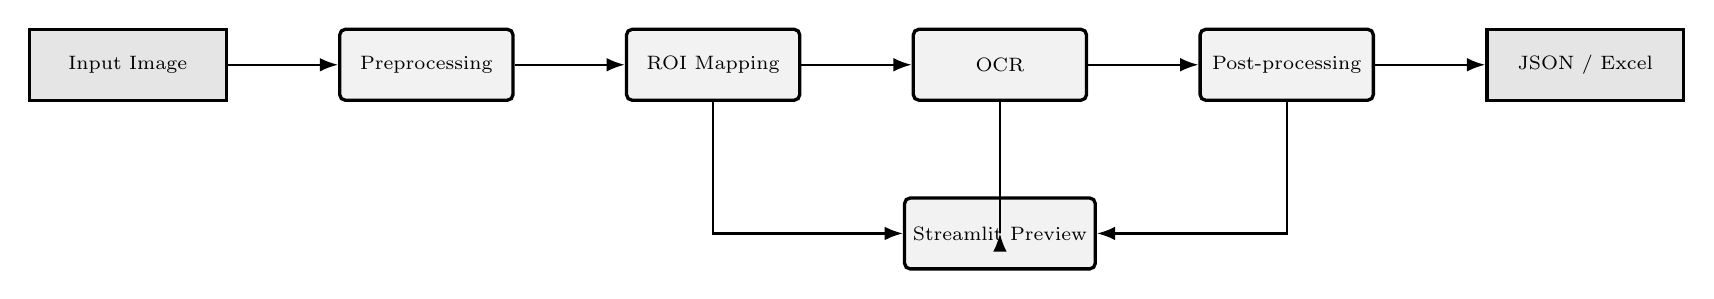
\begin{tikzpicture}[
  node distance=10mm and 14mm,
  >=Latex,
  font=\scriptsize,
  proc/.style={rectangle, rounded corners=2pt, draw=black, fill=gray!10, very thick, inner sep=3pt, align=center, minimum width=2.2cm, minimum height=0.9cm},
  io/.style={rectangle, draw=black, very thick, fill=gray!20, inner sep=3pt, align=center, minimum width=2.5cm, minimum height=0.9cm},
  arr/.style={-Latex, thick}
]

% Main pipeline
\node[io] (input) {Input Image};
\node[proc, right=of input] (prep) {Preprocessing};
\node[proc, right=of prep] (roi) {ROI Mapping};
\node[proc, right=of roi] (ocr) {OCR};
\node[proc, right=of ocr] (post) {Post-processing};
\node[io, right=of post] (output) {JSON / Excel};

% Streamlit below
\node[proc, below=12mm of ocr] (ui) {Streamlit Preview};

% Connections
\draw[arr] (input) -- (prep);
\draw[arr] (prep) -- (roi);
\draw[arr] (roi) -- (ocr);
\draw[arr] (ocr) -- (post);
\draw[arr] (post) -- (output);

% Streamlit tap
\draw[arr] (roi) |- (ui);
\draw[arr] (ocr) |- (ui);
\draw[arr] (post) |- (ui);

\end{tikzpicture}
}
\caption{Simplified graphical abstract of the document processing pipeline.}
\label{fig:pipeline}
\end{figure}


% ---------------------------------------------------------------------------------------------------------------


\chapter{State of the art/Related work}
\label{chapter:stateOfArt}

Document digitization and text extraction have been long-standing goals in intelligent automation.  
Traditional OCR-based systems have evolved from deterministic template matching toward adaptive, machine-learning-based methods.

\section{Classical approaches}
Early OCR engines such as \textbf{Tesseract}~\cite{Smith2007} and \textbf{ABBYY FineReader}~\cite{ABBYYFineReader} rely on rule-based character segmentation and pattern matching.  
They achieve good results on printed text but degrade when faced with handwriting, noise, or low contrast.  
Classical preprocessing --- deskewing, thresholding, and denoising --- remains crucial for improving recognition quality~\cite{Niblack1985,Sauvola2000}.

\section{Modern learning-based methods}
Recent advances use deep learning to recognize both printed and cursive text.  
Libraries like \textbf{EasyOCR}~\cite{JaidedAI2020} employ convolutional networks trained on multilingual datasets to perform character detection and recognition jointly.  
In contrast to Tesseract, EasyOCR generalizes better to varied fonts and handwritten inputs, making it suitable for heterogeneous administrative documents.  
Other research directions, such as \textbf{LayoutLM}~\cite{Xu2020} and \textbf{DocFormer}~\cite{Appalaraju2021}, combine text with spatial layout embeddings, but these models require large datasets and substantial compute power.

\section{Hybrid and practical solutions}
For specialized, small-data domains such as Romanian CNAS certificates, lightweight hybrid approaches are preferable.  
Our solution combines classical image preprocessing (\textbf{OpenCV}~\cite{Bradski2000}) with a deep-learning OCR engine (\textbf{EasyOCR}~\cite{JaidedAI2020}), controlled by a region-based extraction logic defined through an ROI map.  
This design keeps inference deterministic, fast, and interpretable while maintaining adaptability to new templates.

\section{Tools and technologies used}
\begin{itemize}
  \item \textbf{OpenCV:} grayscale conversion, deskewing, thresholding, and image normalization~\cite{Bradski2000}.
  \item \textbf{EasyOCR:} recognition engine for printed and handwritten text~\cite{JaidedAI2020}.
  \item \textbf{Streamlit:} front-end framework for fast UI prototyping and visualization~\cite{Streamlit2023}.
  \item \textbf{Pandas \& OpenPyXL:} for structured data management and Excel export~\cite{McKinney2010,OpenPyXL2024}.
  \item \textbf{Python:} main programming language ensuring modularity and cross-platform compatibility~\cite{PythonDocs}.
\end{itemize}

Compared to previous rule-based systems, this hybrid pipeline delivers robust performance with limited data, minimal manual configuration, and full reproducibility.


% ---------------------------------------------------------------------------------------------------------------


\chapter{Investigated approach}
\label{chapter:proposedApproach}

\section{Overview}
The system operates by mapping a predefined set of normalized regions of interest (ROIs) onto the uploaded image, cropping each region, and running OCR individually.  
This ensures consistent extraction even if the document is slightly misaligned or scaled.  

\paragraph{ROI grid definition and mapping.}
Rectangles are manually annotated on an aligned certificate image of fixed size (1400$\times$1980).  
Each rectangle is stored as normalized coordinates $[t, l, b, r]$ in a JSON file (\texttt{roi\_map.json}).  
When a new image is uploaded, these coordinates are scaled to the image's actual dimensions.  
Each cropped region is passed to EasyOCR~\cite{JaidedAI2020}, and the recognized text is postprocessed according to its field type.

\begin{algorithm}[H]
\caption{ROI-driven OCR pipeline (as implemented)}
\begin{algorithmic}
  \STATE Load normalized ROI map $\mathcal{R}$ from \texttt{roi\_map.json}
  \STATE Read input image $I$, convert to grayscale, deskew, and threshold
  \FOR{each field $k$ with ROI $(t,l,b,r) \in \mathcal{R}$}
     \STATE $(y_1,y_2,x_1,x_2)\leftarrow \text{scale}(t,l,b,r,\text{height}(I),\text{width}(I))$
     \STATE $C \leftarrow I[y_1\!:\!y_2,\,x_1\!:\!x_2]$
     \STATE $s \leftarrow \text{EasyOCR}(C)$
     \STATE $v_k \leftarrow \text{postprocess}(s, \text{kind}(k))$
  \ENDFOR
  \STATE \textbf{return} JSON dictionary $\{k \mapsto v_k\}$ and preview image with ROI overlays
\end{algorithmic}
\end{algorithm}

\paragraph{Per-field postprocessing}
\begin{itemize}
  \item \textbf{digits:} keep numeric characters, enforce expected length (e.g., CNP = 13 digits).
  \item \textbf{date:} regex-based parsing and normalization to ISO format.
  \item \textbf{text:} trim, preserve diacritics, remove duplicates.
  \item \textbf{checkbox:} classify as checked/unchecked based on average pixel intensity.
\end{itemize}

\section{Validation and output}
After all ROIs are processed, the system validates the extracted values using regular expressions and consistency checks (e.g., date intervals, numeric formats).  
The results are displayed in the Streamlit interface~\cite{Streamlit2023}, shown as both JSON and a pandas~\cite{McKinney2010} table, and optionally exported as an Excel file via OpenPyXL~\cite{OpenPyXL2024}.

\section{Software architecture}
The implementation follows a modular structure:
\begin{itemize}
  \item \texttt{ocr\_utils.py} - ROI scaling, OCR execution, postprocessing, validation.
  \item \texttt{app.py} - Streamlit UI, language switching (English/Romanian), and Excel export.
  \item \texttt{roi\_map.json} - ROI definitions.
\end{itemize}
Components are loosely coupled, and the OCR engine can be replaced or retrained independently.

\noindent \textit{AI serving:} the OCR component is \textbf{embedded} in the application (no external microservice); model weights are loaded at runtime by EasyOCR.


\section{Debugging and testing}
During development, a dedicated debugging script (\texttt{debug\_rois.py}) crops all regions of interest (ROIs) from the aligned certificate template and saves them to disk for visual verification.  
This process ensures that ROI coordinates are correctly aligned with the target document layout before running OCR.  

The Streamlit interface itself serves as a real-time visualization and testing environment: each uploaded image is processed, and detected text regions are overlaid and displayed interactively for inspection.  
Formal validation tests (e.g., for CNP or date formats) are planned as future improvements.

\noindent \textit{Iterative perspective:} ROI coordinates were adjusted iteratively based on the Streamlit preview until misalignments were eliminated, after which the ROI map was fixed and versioned.


\section{Development environment.}
The application was implemented in \textbf{Python}~\cite{PythonSoftwareFoundation2024} using the \textbf{Visual Studio Code} editor~\cite{VSCode2024} on Windows 11.  
Development used a local \texttt{venv} virtual environment, with dependencies managed via a \texttt{requirements.txt} file.  
Bugs were identified through ROI misalignment inspection, logging OCR outputs, and verifying extracted field validity during live runs in the Streamlit interface.  
Average workload during testing was below 8 seconds per certificate on a standard laptop CPU.

\section{Versioning and Continuous Delivery}

The project was developed collaboratively in a single \textbf{Git} repository, which contains both the application code and documentation.  
Version control was used to track progress, synchronize work between team members, and maintain a clean commit history.  

All testing and debugging were performed locally in a controlled \texttt{venv} environment.  
Once validated, updates were committed and pushed to the shared repository, ensuring all members had the latest working version.  
This simple yet effective workflow provided continuous integration at the local level and reproducible delivery through Git.


% ---------------------------------------------------------------------------------------------------------------


\chapter{Application (numerical validation)}
\label{chapter:application}

\section{Methodology}
The evaluation focuses on the correctness of extracted fields and runtime performance.  
Three questions guided the experiments:
\begin{enumerate}
  \item How accurately are key fields (Series, Number, CNP, Dates, Diagnostic Code) extracted from typical CNAS certificates?
  \item How robust is the ROI scaling under skew and resolution changes?
  \item What is the end-to-end runtime for a single document?
\end{enumerate}

\paragraph{Testing scope.}
We conducted (i) \textbf{data testing} by validating each field against expected formats (digits, dates, lengths), 
(ii) \textbf{integration testing} by running end-to-end flows (UI upload $\rightarrow$ ROI $\rightarrow$ OCR $\rightarrow$ Excel export) on multiple images, 
and (iii) \textbf{AI quality testing} by computing field-wise extraction accuracy and checkbox recognition accuracy against manually verified ground truth.

\section{Data}
A dataset of 10 anonymised certificates was used.
All certificates share the CNAS form layout but differ slightly in proportions.  
Fields were annotated manually to verify accuracy.  
Images were stored in a versioned data folder to ensure reproducibility.

\noindent \textit{Storage rationale:} a simple, versioned folder structure (``data/'' and ``results/'') was preferred over a data warehouse or lake due to the small dataset size and the need for quick, local iteration.


\section{Results}
\begin{table}[htbp]
\centering
\caption{Summary of extraction performance.}
\begin{tabular}{l c}
\hline
Metric & Value \\
\hline
Field extraction accuracy (printed text) & 85-90\% \\
Field extraction accuracy (mixed text) & 60-65\% \\
Checkbox recognition accuracy & 100\% \\
Average runtime / document & $<$ 8 s \\
\hline
\end{tabular}
\end{table}

The ROI mapping proved stable across all evaluated certificate samples that followed the standard CNAS layout.  
Most recognition errors appeared in low-contrast regions or handwritten zones, particularly for diagnostic codes and partially filled checkboxes.

\section{Discussion}
The results confirm that the hybrid, ROI-driven pipeline is effective for structured document extraction.  
While EasyOCR's handwritten recognition occasionally misclassifies letters, the overall performance is satisfactory given the small dataset and real-world noise.  
Future work will focus on dynamic ROI correction using contour detection and on integrating a confidence-based verification layer.

\section{Experiments tracking}
All test results were stored directly in the shared Git repository for traceability.  
Each experiment produced an Excel file saved under the \texttt{results/} folder, containing the extracted fields and manual validation data.  
This folder served as a simple yet effective tracking mechanism, allowing all team members to compare outputs and verify improvements across commits.  

Given the small dataset and deterministic OCR pipeline, no external experiment-tracking tools (e.g., DVC or MLflow) were required.




% ---------------------------------------------------------------------------------------------------------------


\chapter{SWOT Analysis}
\label{chapter:swot}


% ---------------------------------------------------------------------------------------------------------------


\chapter{Conclusion and future work}
\label{chapter:concl}

Try to emphasise the strengths and the weaknesses of your approach.
What are the major shortcomings of your current method? For each shortcoming, propose additions or enhancements that would help overcome it. 

Briefly summarize the important results and conclusions presented in the paper. 

\begin{itemize}
	\item What are the most important points illustrated by your work? 
	\item How will your results improve future research and applications in the area? 
\end{itemize}


% ---------------------------------------------------------------------------------------------------------------


\bibliographystyle{plain}
\bibliography{BibAll}

\end{document}